\section{Baryons and Mesons as Composite Field States}

\begin{table}[ht]
\centering
\begin{tabular}{lcc}
\hline
\textbf{Property} & \textbf{Standard Model} & \textbf{GCFT} \\
\hline
Ontology         & Quarks/gluons bound by gauge fields & Multi-node $\Xi$-field knots \\
Quarks           & Fundamental particles, color-charged & Partial phase nodes, not free \\
Gluons           & Force-mediating bosons  & Torsion harmonization, no exchange \\
Mass origin      & Confinement, Higgs      & Coherence compression, knot geometry \\
Decay            & Weak/strong mediation   & Phase-lock breakdown in field \\
Stability        & QCD confinement rules   & Knot memory and symmetry-locking \\
\hline
\end{tabular}
\caption{Baryons and mesons: Standard Model vs. GCFT.}
\label{tab:baryon_gcft_compare}
\end{table}

In GCFT, baryons and mesons are not composed of fundamental particles like quarks and gluons. Instead, they emerge as multi-node field structures — composite resonance formations stabilized by symmetry-locking and coherence recycling within the $\Xi$ field. What the Standard Model interprets as constituent quarks are partial phase structures: incomplete torsion configurations whose interactions define the larger coherence structure.

\subsection{Quarks as Partial Phase Nodes}

GCFT reinterprets quarks as \emph{non-stable} subresonances — regions of concentrated phase asymmetry within a larger resonance knot. They do not exist independently, but only as parts of baryonic or mesonic structures. This explains quark confinement without requiring a separate color charge theory.

\subsection{Protons and Neutrons: Compression Trios}

The proton and neutron are each stabilized trios of torsional compression zones — a resonance of three interacting $\Xi$-phase nodes. Their apparent mass difference emerges from the degree of internal compression tension and coherence drag.

\begin{itemize}
  \item \textbf{Proton}: Long-term stable, lowest-energy configuration of three-phase-locked nodes.
  \item \textbf{Neutron}: Slightly higher energy, with internal phase asymmetry leading to delayed decoherence.
\end{itemize}

Their topological structure resembles a $\Xi$-knot triangle — each “quark” a convergence point of phase tension and memory. Gluon exchange is replaced by local $\Xi$ torsion harmonization.

\begin{table}[ht]
\centering
\begin{tabular}{lcccc}
\hline
\textbf{Particle} & \textbf{Mass (MeV)} & \textbf{Luxions} & \textbf{GCFT Topology} & \textbf{Stability/Decay} \\
\hline
Proton ($p$)     & 938.3   & $6.89 \times 10^7$    & 3-node $\Xi$-knot       & Stable \\
Neutron ($n$)    & 939.6   & $6.91 \times 10^7$    & 3-node $\Xi$-knot w/ drift & Decay (880\,s) \\
Pion ($\pi^+$)   & 139.6   & $1.03 \times 10^7$    & 2-node braid            & Snap decay \\
Kaon ($K^+$)     & 493.7   & $3.63 \times 10^7$    & Braid + compressed node & Leak, then snap \\
Rho ($\rho$)     & 775.3   & $5.70 \times 10^7$    & Multi-lobed braid       & Short-lived \\
\hline
\end{tabular}
\caption{GCFT mapping for representative baryons and mesons. All hadron masses emerge from multi-node resonance in the $\Xi$-field, not from constituent quark masses.}
\label{tab:hadron_gcft}
\end{table}

\paragraph{GCFT Field Model for a Proton (Conceptual):}
Three phase-locked nodes in $\Xi$:
\[
\Xi_{\text{proton}}(r, \theta) \approx \sum_{i=1}^3 f_i(r) e^{i n_i \theta}
\]
where $n_i$ encodes local phase winding for each node. The field energy density sets the mass; symmetry-locking sets stability.

\begin{figure}[ht]
\centering
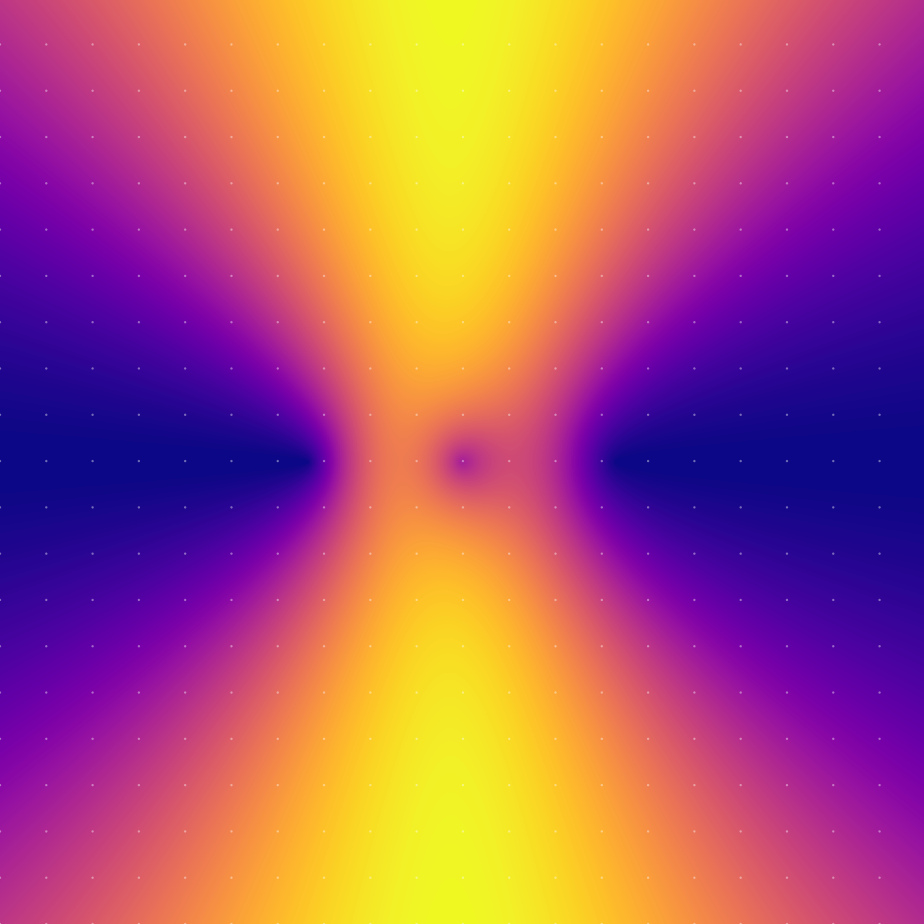
\includegraphics[width=0.6\textwidth]{figures/deuterium_modulus_vector_overlay.png}
\caption{Ξ-Field Structure of Deuterium. Compression nodes from a $\Xi$-proton, $\Xi$-neutron, and shared $\Xi$-electron form a stable three-body resonance.}
\label{fig:deuterium_field}
\end{figure}

\subsection{Mesons: Field Rebound and Decoherence Pulses}

Mesons are not quark-antiquark pairs but transient rebound states — pulse solutions in the coherence field that arise during field unwinding or partial node decomposition.

\begin{itemize}
  \item \textbf{Pions}: $\Xi$-shell decompressors — smoothing pulses emitted during field tension discharge. Their low mass and short lifetime follow from their phase role, not constituent masses.
  \item \textbf{Kaons}: Failed $\Xi$-core rebuilds — memory-trapped field loops that decay via coherence slippage.
  \item \textbf{Rho, Phi, etc.}: Higher-order rebound loops with more intricate internal $\Xi$ tension folding.
\end{itemize}

\begin{figure}[ht]
\centering
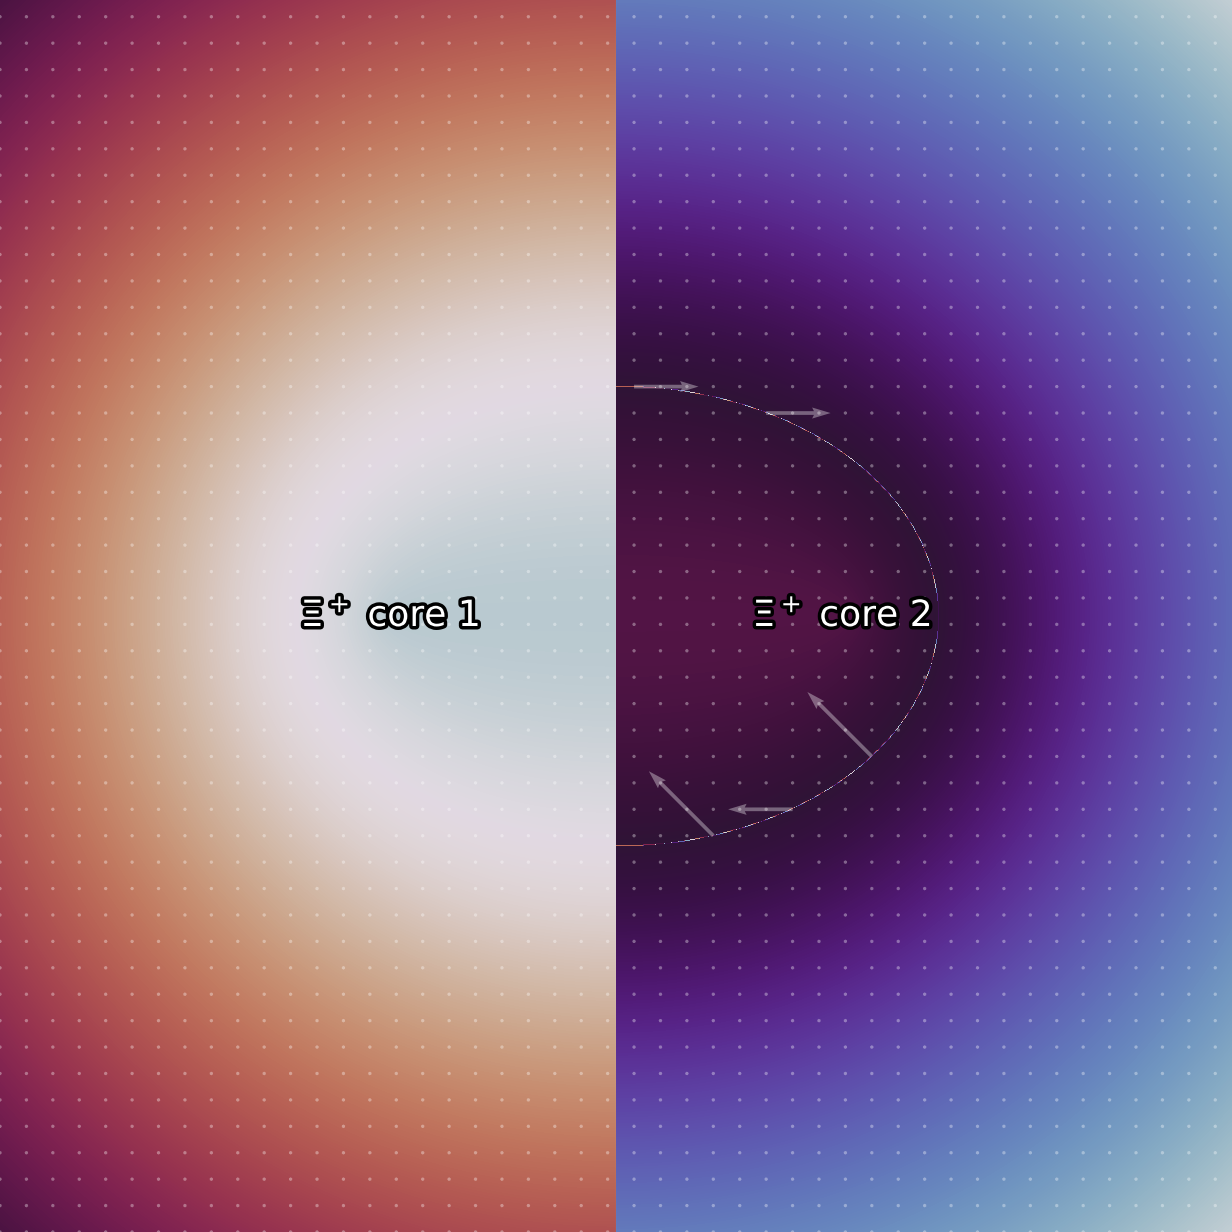
\includegraphics[width=0.6\textwidth]{figures/pion_phase_final.png}
\caption{Ξ-Phase Landscape of the $\pi^+$ Meson. Two $\Xi^+$ lobes form a resonance structure with a coherent rebound zone, illustrating phase interference without internal mass lock.}
\label{fig:pion_phase}
\end{figure}

\begin{figure}[ht]
\centering
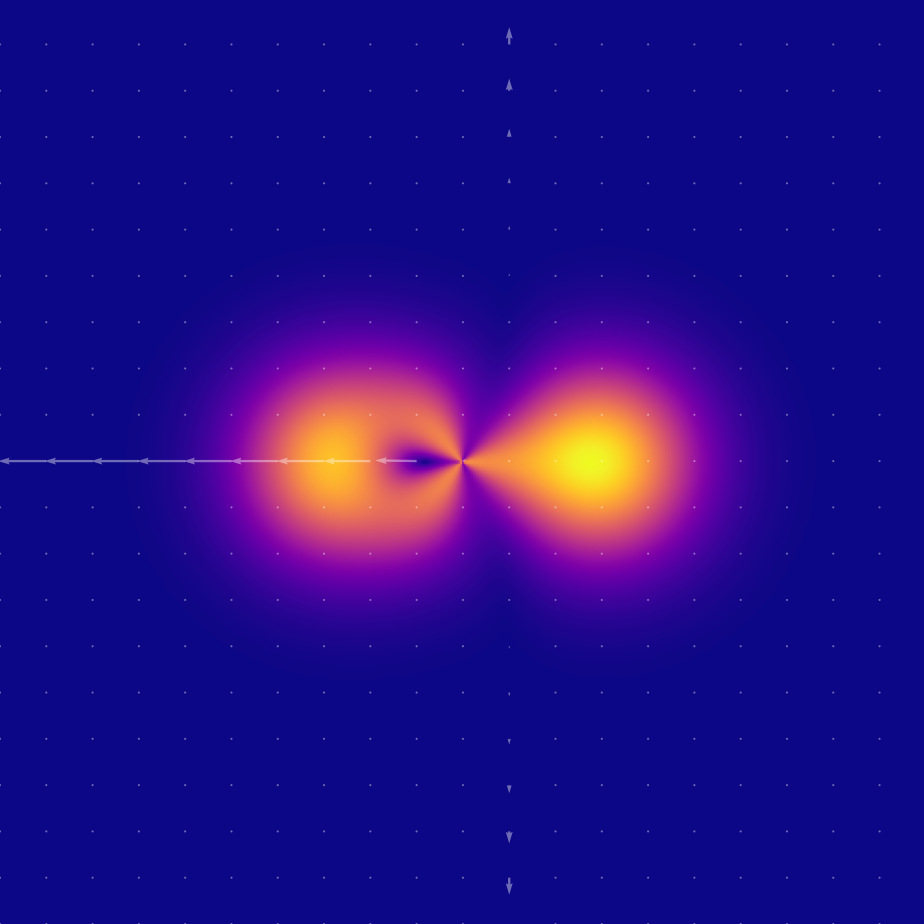
\includegraphics[width=0.48\textwidth]{figures/xi_kaon_field_overlay.png}
\caption{Ξ-Field Structure of the Kaon. An asymmetric rebound configuration with partial phase restoration and a coherence trap at the center. The field does not fully re-lock, leading to instability and decay.}
\label{fig:kaon_field}
\end{figure}

\begin{figure}[ht]
\centering
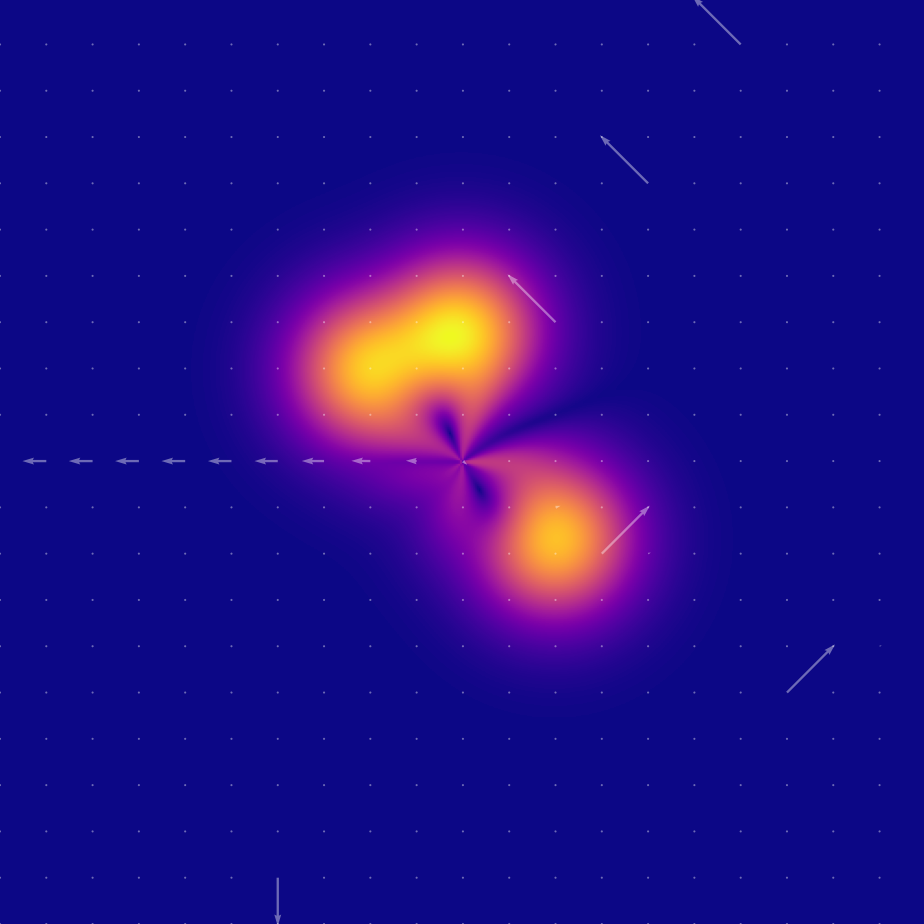
\includegraphics[width=0.48\textwidth]{figures/xi_rho_field_overlay.png}
\caption{$\Xi$-Field Configuration of the $\rho$ Meson. A higher-order rebound state with multi-lobed interference and internal phase folds. The structure’s short lifetime reflects instability in its coherence distribution.}
\label{fig:rho_field}
\end{figure}

\subsection{\texorpdfstring{Decay Channels and $\Xi$ Phase Logic}{Decay Channels and Xi Phase Logic}}

Mesons and baryons decay not via force mediation, but via phase-lock breakdown. As a composite $\Xi$ structure exceeds its stability margin (due to energy input, drift, or interference), the field reconfigures into simpler standing waves. This explains particle decays without invoking weak force bosons — the $\Xi$ field resolves coherence imbalance on its own.

\subsection{Implications}

GCFT dissolves the distinction between fermions and bosons as fundamental vs composite. All hadrons are standing $\Xi$ structures with different phase topologies and memory paths. Their lifetimes, masses, and decay pathways follow naturally from the geometry of $\Xi$ coherence, not from gauge theory or fractional charges.

\begin{figure}[ht]
\centering
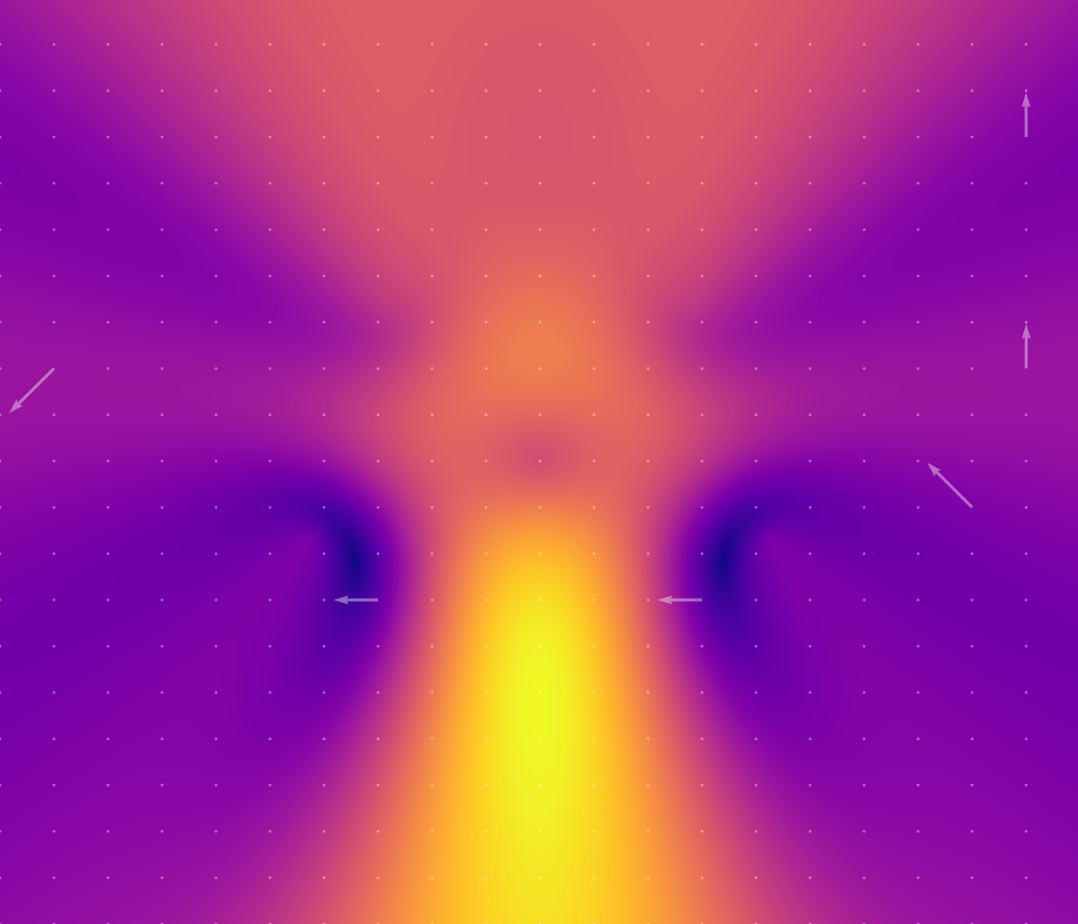
\includegraphics[width=0.48\textwidth]{figures/tritium_modulus_vector_overlay.png}
\caption{GCFT Field Topology of Tritium. A five-body coherence trap formed by one $\Xi$-proton, two $\Xi$-neutrons, and two $\Xi$-electrons.}
\label{fig:tritium_field}
\end{figure}

\paragraph{GCFT Predictions for Hadrons:}
\begin{itemize}
  \item All baryon and meson masses are set by node topology, not quark content.
  \item No free quarks exist—confinement arises naturally from field geometry.
  \item Baryon decay lifetimes are determined by phase drift and coherence loss, not by weak force bosons.
  \item GCFT predicts observable time delays and low-frequency chirps during hadronic decay, measurable in precision timing experiments.
  \item Any discovery of stable multi-quark exotics outside allowed knot topologies would falsify this framework.
\end{itemize}
